%% LyX 2.0.5.1 created this file.  For more info, see http://www.lyx.org/.
%% Do not edit unless you really know what you are doing.
\documentclass[12pt]{report}
\usepackage{mathptmx}
\renewcommand{\familydefault}{\rmdefault}
\usepackage[T1]{fontenc}
\usepackage[latin9]{inputenc}
\usepackage[a4paper]{geometry}
\geometry{verbose,tmargin=2cm,bmargin=2cm,lmargin=2cm,rmargin=2cm,headheight=1cm,headsep=1cm,footskip=1cm}
\setcounter{secnumdepth}{2} % Changed from 3 to 2. 0-chapter 1-section 2-subsection 
\setcounter{tocdepth}{2} % Changed from 3 to 2. 0-chapter 1-section 2-subsection 
\setlength{\parskip}{\medskipamount}
\setlength{\parindent}{0pt}
\usepackage{verbatim}
\usepackage{pdfpages}
\usepackage{graphicx}
\usepackage{setspace}
\usepackage[numbers]{natbib}
\usepackage{nomencl}
% the following is useful when we have the old nomencl.sty package
\providecommand{\printnomenclature}{\printglossary}
\providecommand{\makenomenclature}{\makeglossary}
\makenomenclature
\doublespacing

\makeatletter

%%%%%%%%%%%%%%%%%%%%%%%%%%%%%% LyX specific LaTeX commands.
\providecommand{\LyX}{L\kern-.1667em\lower.25em\hbox{Y}\kern-.125emX\@}
%% Because html converters don't know tabularnewline
\providecommand{\tabularnewline}{\\}
%% A simple dot to overcome graphicx limitations
\newcommand{\lyxdot}{.}


%%%%%%%%%%%%%%%%%%%%%%%%%%%%%% User specified LaTeX commands.
\usepackage{tauthesis}
\usepackage[font={small,bf}, labelfont={small,bf}, margin=1cm]{caption}
\usepackage{titlesec}
\newcommand{\hsp}{\hspace{20pt}}
\titleformat{\chapter}[hang]{\Huge\bfseries}{\thechapter\hsp}{0pt}{\Huge\bfseries}


\Title{\textbf{Thesis Title}}
\Author{First Last}
\Year{August 2013}
\Supervisor{Prof. Alex Liberzon}
\Department{School of Mechanical Engineering}
\Degree{Master of Science}
% \Degree{Doctor of Philosophy}

\makeatother

\begin{document}
\begin{comment}
This is Micheal JasonSmith's uocthesis example ported to \LyX{} by
Etienne Lalibert� (etiennlaliberte@gmail.com).

Alex Liberzon (alex.liberzon@gmail.com) modified it to the Tel Aviv
University format, with the logo of the Faculty of Engineering. Change
the file taulogo.png to get the logo of your department.

Go to \textsf{Document > Settings > \LaTeX{} preamble} to modify the
\textsf{Title, Author, Year, Supervisor, Department} fields.

Default processor is now DVIPDFM - but if you can choose something
else, try PDFLATEX and XELATEX - sometimes these are a bit faster. 
\end{comment}


\prelimpages

\titlepage

\acknowledgments{I would like to thank my ...}

\begin{comment}
Split the thesis into separate chapters. Use \textbackslash{}include
mode to include the separate files.

Use \LyX{} Table of Contents, List of Figures, List of Tables and
Nomenclature automatics to include them in the thesis. Double - click
on each item to change the default level of contents, move the chapters
up/down and so on.
\end{comment}

\cleardoublepage
\setcounter{page}{1} % Start preliminary pages numbering (roman numerals).

\chapter*{Abstract}

Here comes the 1-2 pages long abstract of the thesis in English.  

    

\tableofcontents{}

\listoffigures

\listoftables

\printnomenclature{}

\textpages

%% LyX 2.0.5.1 created this file.  For more info, see http://www.lyx.org/.
%% Do not edit unless you really know what you are doing.
\documentclass[twoside,english]{report}
\usepackage[T1]{fontenc}
\usepackage[latin9]{inputenc}
\setcounter{secnumdepth}{3}
\setcounter{tocdepth}{3}
\usepackage[active]{srcltx}
\usepackage{verbatim}
\usepackage{graphicx}
\usepackage{setspace}
\usepackage[numbers]{natbib}
\doublespacing

\makeatletter

%%%%%%%%%%%%%%%%%%%%%%%%%%%%%% LyX specific LaTeX commands.
\providecommand{\LyX}{L\kern-.1667em\lower.25em\hbox{Y}\kern-.125emX\@}
%% Because html converters don't know tabularnewline
\providecommand{\tabularnewline}{\\}

\makeatother

\usepackage{babel}
\begin{document}

\chapter{Introduction}

Introduction chapter. We recommend using bibtex to manage your list
of references and organize the literature citation style. All is done
automatically by \LyX{}. While working on separate files it's useful
to include the bibtex file in each file locally, in the yellow note
(so it's recognized by the compiler but not complaining if you run
the Master document). 


\section{Figures}

Include figures as usual, first Insert -> Float -> Figure, then Insert
-> Graphics. 

Use cross-reference option to talk about Fig. \ref{fig:Some-caption-for}

\begin{figure}
\begin{centering}
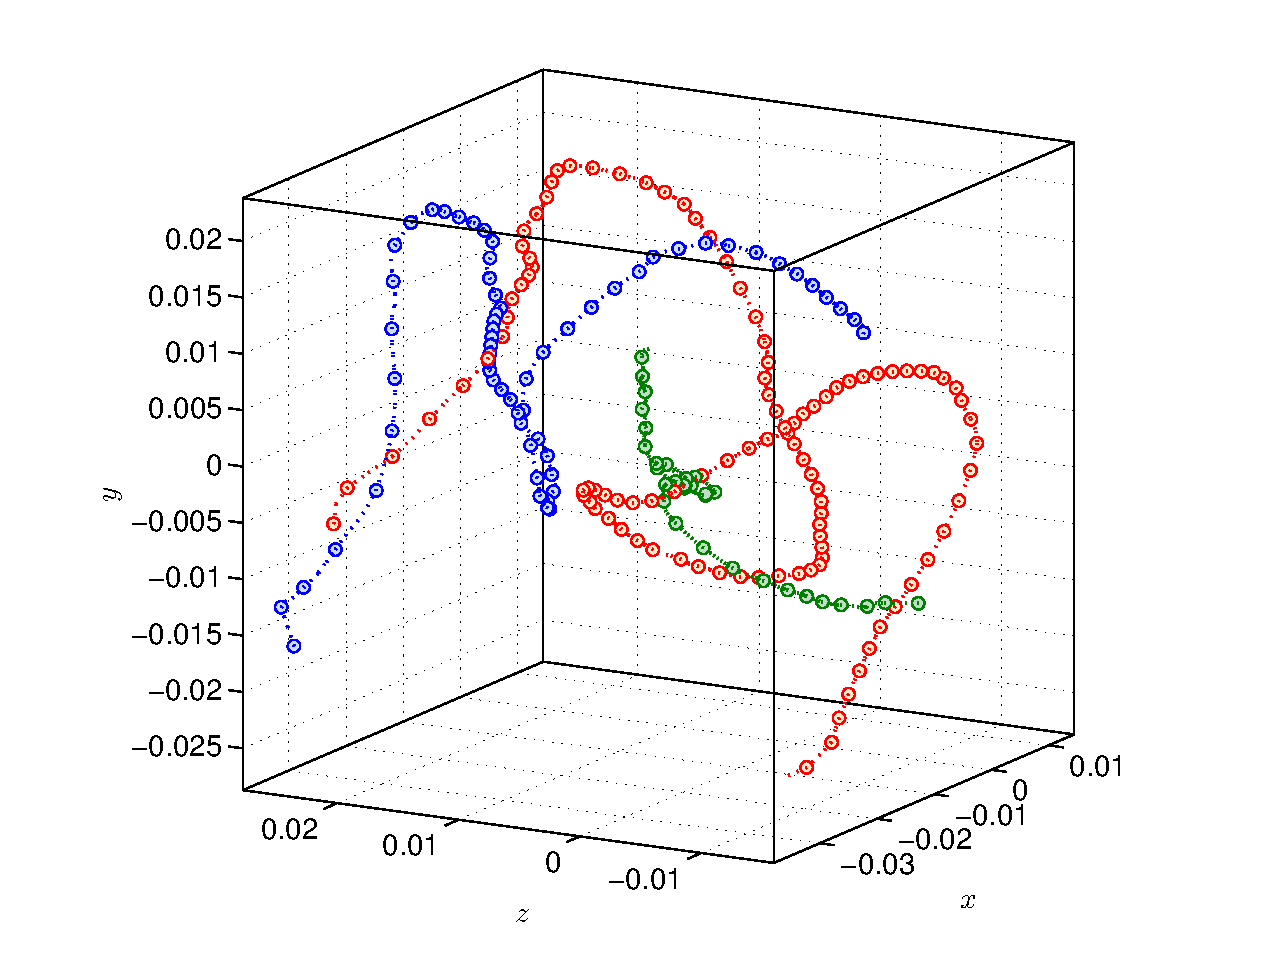
\includegraphics[width=0.8\textwidth]{few_long_trajectories}
\par\end{centering}

\caption{Some caption for the figure. Don't forget adding label to the figure
and later using the cross-reference to it. \label{fig:Some-caption-for}}


\end{figure}



\section{Tables}

\begin{table}
\begin{tabular}{|c|c|c|}
\hline 
row 1 & cell 1 & cell 2\tabularnewline
\hline 
\hline 
row 2 & cell 1 & cell 2\tabularnewline
\hline 
\end{tabular}

\caption{Table float first using Insert - > Float -> Table}


\end{table}


\begin{comment}
Use: Insert Note -> Insert List/TOC -> Bibtex Bibliography
\end{comment}




\begin{comment}
Then in the text you can use Insert citation (use the icon for the
quick use)
\end{comment}



\section{Citations}

The file references.bib in this folder is an example of how to organize
the bibliography database. It is very simple to add a reference/citation
to one of the items in the bibliography list, e.g. see the best source
of information regarding the OpenPTV origins: \citet{Dracos1996}.
Simply use: Insert -> Citation and choose from the list on the left.
Add it to the list on the right and you'll be able to choose the format
of author-year or author-number or just number to the references.
At the same time, at the end of the document you'll find References
chapter with all the cited references automatically chosen and included. 
\end{document}


\bibliographystyle{plainnat}
\bibliography{references}

\appendix

\chapter{Appendix title}

Appendix is just a different type of Section - it's included at the
end of the document (after the bibliography or list of references)
and before the Hebrew part and it's numbered in a different manner. 


\newpage{}

\begin{comment}
It is possible to create the Hebrew part in \LyX{}, but this is less
of our concern. Any typesetting software like \LyX{} (or Word or OpenOffice)
is as good for this purpose. After creating the PDF file from the
Hebrew document, include it here using the Insert -> File -> External
material -> PDFpages (one of the options). See the example below. 
\end{comment}



\includepdf[pages=-]{hebrew_part}
\end{document}
